\documentclass{report}
\title{Diffusion of Proteins on Cell Membranes \\ 1D Finite Element Method}
\author{Aaron Kaw}
\date{}

\usepackage{amsmath}
\usepackage{amsfonts}
\usepackage{physics}
\usepackage{nicefrac}
\usepackage{tabularx}
\usepackage{parskip}
\usepackage[hidelinks]{hyperref}
\usepackage{graphicx}

\graphicspath{
	{../imgs/cell_biology/}
}

\newcommand\Par[1]{{ \left({#1}\right) }}
\newcommand\Brack[1]{{ \left[{#1}\right] }}
\newcommand\Brace[1]{{ \left\{{#1}\right\} }}
\newcommand\Abs[1]{{ \left\lvert{#1}\right\rvert }}
\newcommand\Angle[1]{{ \left\langle{#1}\right\rangle }}

\newcommand\nf[2]{{ \nicefrac{#1}{#2} }}

\newcommand\bbP{{ \mathbb{P} }}
\newcommand\bbR{{ \mathbb{R} }}
\newcommand\bbZ{{ \mathbb{Z} }}

\newcommand\D{{ D' }}
\newcommand\R{{ R' }}
\newcommand\Rs{{ R'_s }}
\newcommand\Rc{{ R'_c }}
\newcommand\Rv{{ R'_v }}

\newcommand\SA{{ \text{SA} }}
\newcommand\FC{{ \text{FC} }}
\newcommand\KR{{ \text{KR} }}
\newcommand\KRv{{ \text{KRv} }}
\newcommand\KRc{{ \text{KRc} }}

\newcommand\spot{{ \text{spot} }}
\newcommand\ring{{ \text{ring}  }}
\newcommand\conv{{ \text{conv} }}

\newcommand{\ze}{{ \zeta }}

\begin{document}
\maketitle
\tableofcontents

\chapter{Introduction}
\section{Abstract}
Protein delivery to a cell membrane via internal vesicles consists of two alternative fusion modes that contrast in energy expenditure and resource-cost. Thus, identifying a cell's bias to either of the two modes can suggest the process acting in the cell. However, current experimental and observational methods for time-dependent fusion events are limited in resolution, obscuring the differences between the two modes. We model both modes, simulate over the parameters spaces of known values for mammalian cells, and compare the theoretical evolution of the fusion and diffusion process. Failure to distinguish the two modes in simulation with infinite resolution can suggest the impossibility in making distinctions with limited resolution. On the other hand, successful distinctions in simulations can suggest the type of observations that may provide further resolution of the process in the laboratory setting.

\section{Reading}
This document is a detailed description of the biological and experimental background, the mathematical model, programmed implementation, and interpretation of results. The audience is math graduates who have familiarity with the fields of cell biology. Needless to say, the reader can skip to the interpretation at the end of the document.

The first part details the biological background, effectively a literature review giving context for the motivation behind developing the diffusion model derived here.
The second part provides the mathematical derivation of the fusion and diffusion model, approximately to a one-to-one relationship with the biological background given.
The third part gives a summary of the implementation in the Julia programming language, including the application programming interface (API) from a selection of biological parameters.
The fourth part gives an interpretation of the model results, providing rationale for conclusions.

The topic of this document is effectively divided into three ordered stages, found as a structural theme throughout the document:
\begin{enumerate}
	\item Fusion
	\item Diffusion
	\item Observation
\end{enumerate}

\part{Cell and Protein Dynamics}
\chapter{Cell and Protein Biology}
\section{Cell}
Mammalian cells range in volume from 100 to 10'000 micrometers and are surrounded by a largely impermeable membrane with a typical thickness of 4 to 10 nanometers \cite{milo2010bionumbers}. The extremely thin nature of the membrane can be demonstrated by scaling the cell size up to that of a watermelon, where the resulting membrane thickness becomes that of a sheet of paper. This membrane is composed of phospholipids, which have hydrophilic heads and hydrophobic tails as shown in \autoref{fig:phospholipid_membrane}.

\begin{figure}
	\centering
	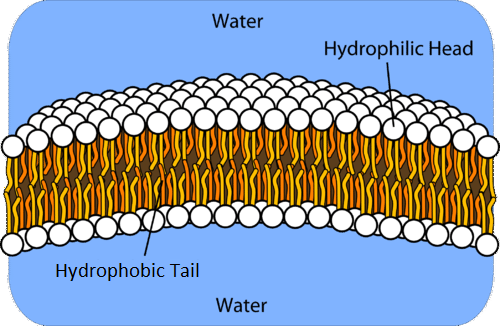
\includegraphics[width = 0.5\textwidth]{phospholipid_membrane.png}
	\caption{Visualisation of the phospholipid structure of cell membranes. Reproduced from \cite{soult2020phospholipids}}
	\label{fig:phospholipid_membrane}
\end{figure}

Phospholipids react to the exposure of water. When a collection of phospholipids are placed in an aqueous environment, the hydrophobic tails are repelled from the water, whilst the heads are attracted to the water \cite{yeagle1978phospholipid}, also illustrated in \autoref{fig:phospholipid_membrane}. Cellular lipid bilayers are also referred to as membranes.

\section{Proteins}
The outer cell membrane is largely impermeable. In order to transport molecules such as glucose and proteins into and out of the cell, other protein structures are integrated into the structure of the membrane. Such proteins appear in many forms including peripheral, channel, integral, and internal, taking up up to 30\% of the membrane surface area. These molecules carry out specific functions and are free to move laterally on the membrane. Thus, one may think of these proteins on cell membranes as objects free to move laterally in a viscous fluid \cite{marrink2019computational} hence the additional nomenclature of plasma membrane.

Some cellular functions the proteins enable include \cite{alberts2002protein}:
\begin{itemize}
	\item transporting materials across the membrane through channels,
	\item catalysing chemical reactions,
	\item receiving and sending chemical signals,
	\item responding to stimuli, and
	\item providing structural support.
\end{itemize}

A visual representation of membrane-embedded proteins is given in \autoref{fig:membrane_proteins}.

\begin{figure}
	\centering
	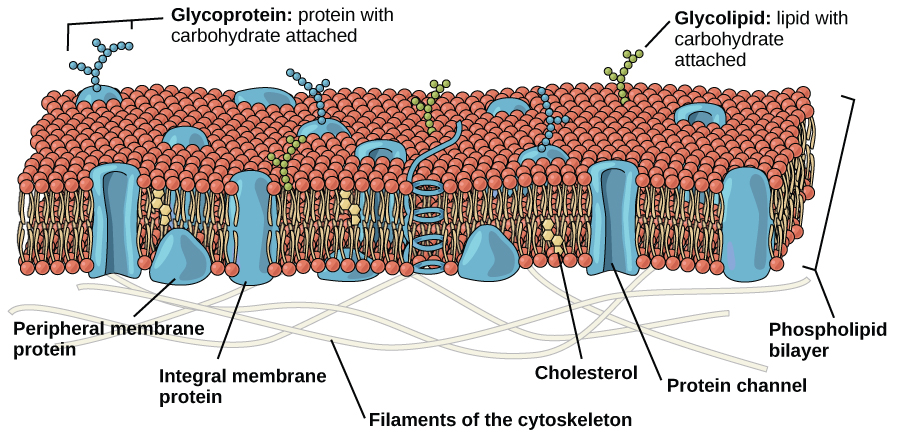
\includegraphics[width = \textwidth]{membrane_proteins.png}
	\caption{A patch of phospholipid bilayer membrane with embedded cellular proteins. Reproduced from \cite{openstax2012plasma}.}
	\label{fig:membrane_proteins}
\end{figure}

\section{Vesicles}
Cells have the capacity to change the amount of membrane-embedded proteins on the outer cell membrane via vesicles \cite{ales2007gene}. Vesicles deliver their contents to different locations inside and outside the cell by merging their membrane with that of the destination, or detaching from their origin. This is possible due to sharing a phosopholipid bilayer design, which likewise carries membrane-embedded proteins.

In a process termed exocytosis, a cell's internal vesicle merges with the cell membrane and the vesicle's internal fluid contents is released to the extracellular volume, such as happens in neural signalling. Additionally, and more importantly for the current study, the fusion delivers the membrane-embedded vesicle contents to the cell [REF].

The reverse process is termed endocytosis, wherein a small section of cell membrane buds into a vesicle, usually containing membrane-embedded and/or internally contained molecules for transport. The vesicle is then transported to the destination. Outside the scope of study, both processes have extracellular equivalents.

The delivery of molecules via vesicles engages in dynamics of membrane fusion. Various other membrane proteins perform roles such as acting as grappling hooks in the initiation of vesicle-cell membrane fusion \cite{han2017multifaceted}. The event itself requires energy due to potential exposure of the lipid tails to the aqueous environment, or the temporary bending of lipid bilayers. Once fusion has begun, one of two known modes are employed \cite{harata2006kiss}.

\subsection{Full-Collapse Fusion}
In the Full-Colapse (FC) Fusion mode, the vesicle membrane bends to conform to the curvature of the cellular membrane, and any membrane-embedded contents naturally become part of the cell membrane. An illustration is given in \autoref{fig:full_collapse_fusion_multiples}.

\begin{figure}
	\centering

	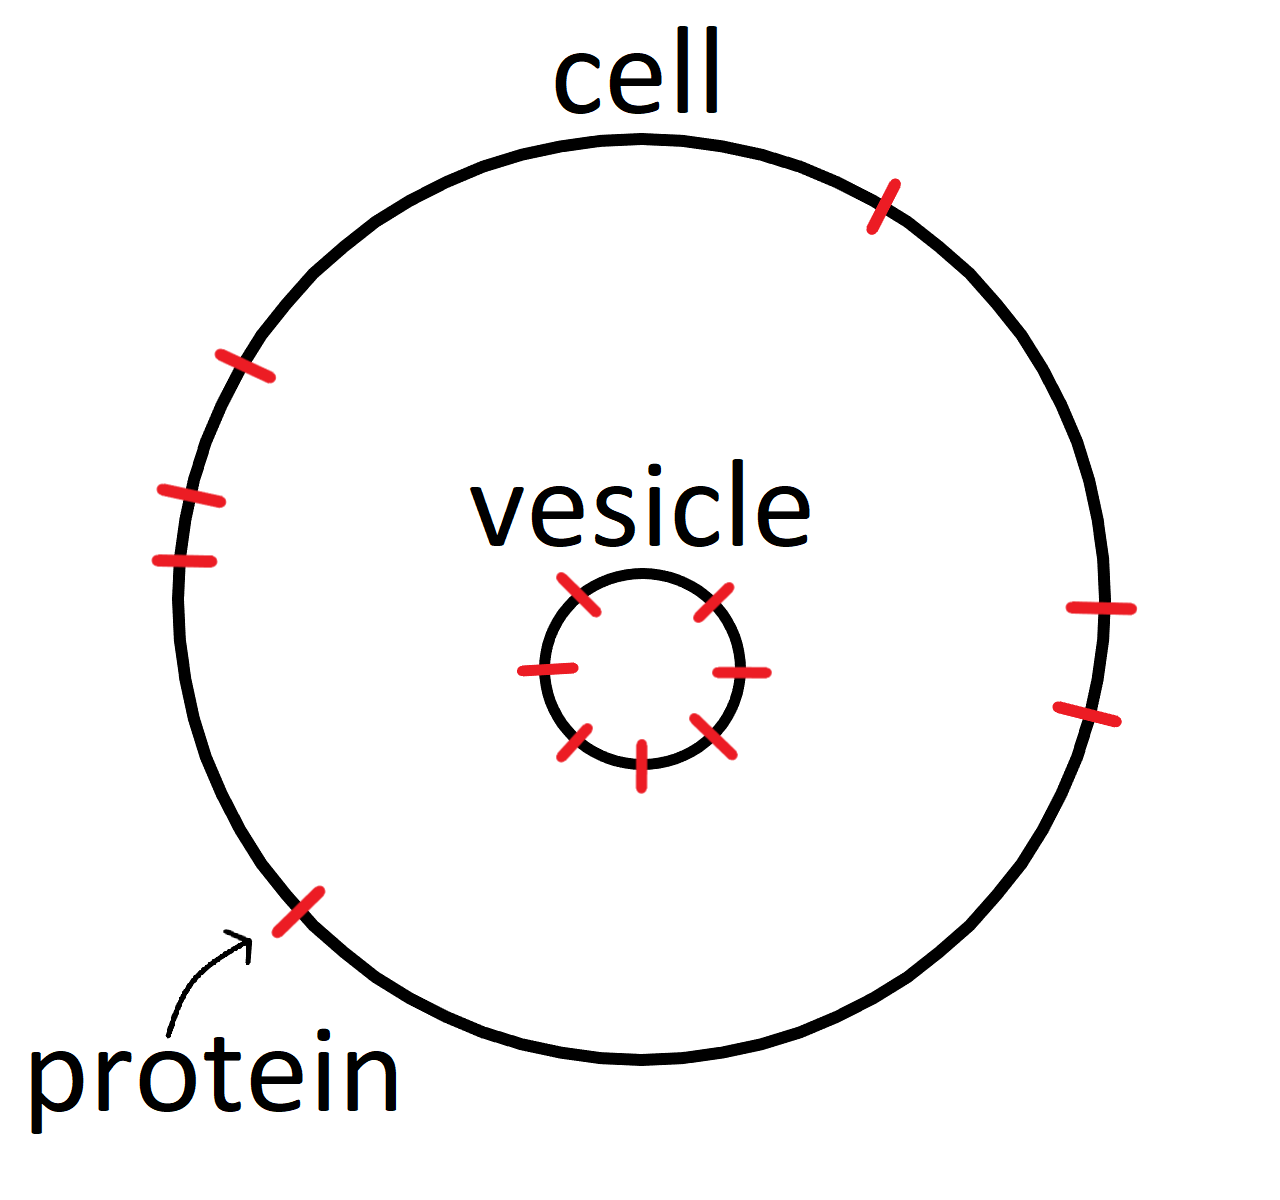
\includegraphics[width = 0.3\textwidth]{fc_fusion/2vesicle.png}
	\includegraphics[width = 0.3\textwidth]{fc_fusion/3transport.png}
	\includegraphics[width = 0.3\textwidth]{fc_fusion/4dock.png}

	\includegraphics[width = 0.3\textwidth]{fc_fusion/5pore.png}
	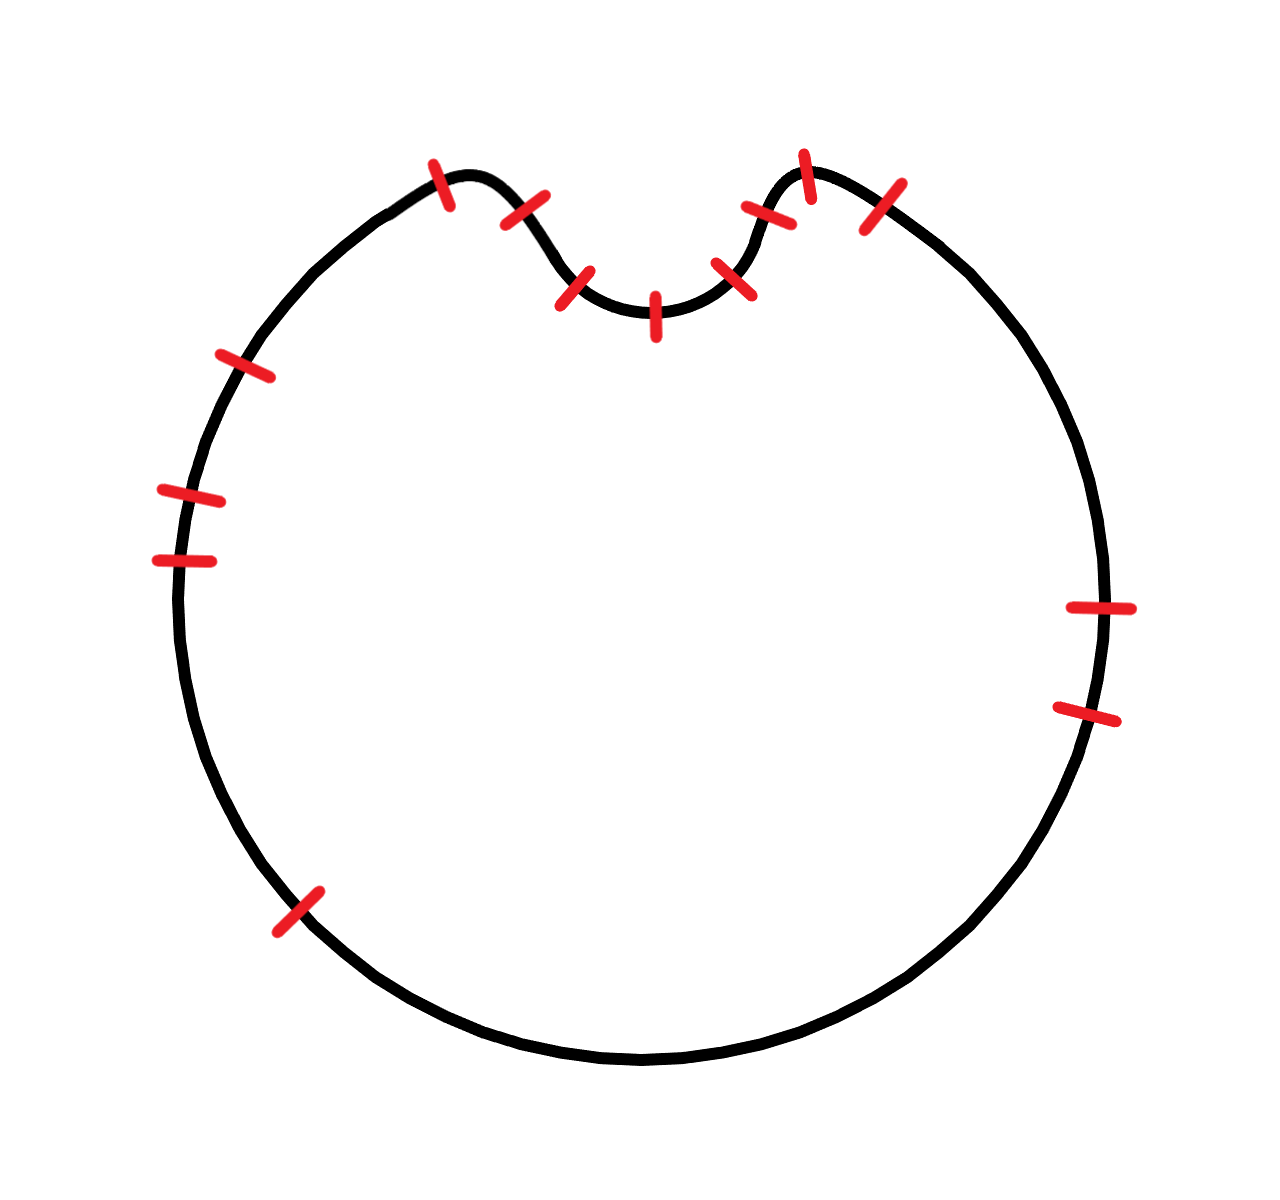
\includegraphics[width = 0.3\textwidth]{fc_fusion/6bend.png}
	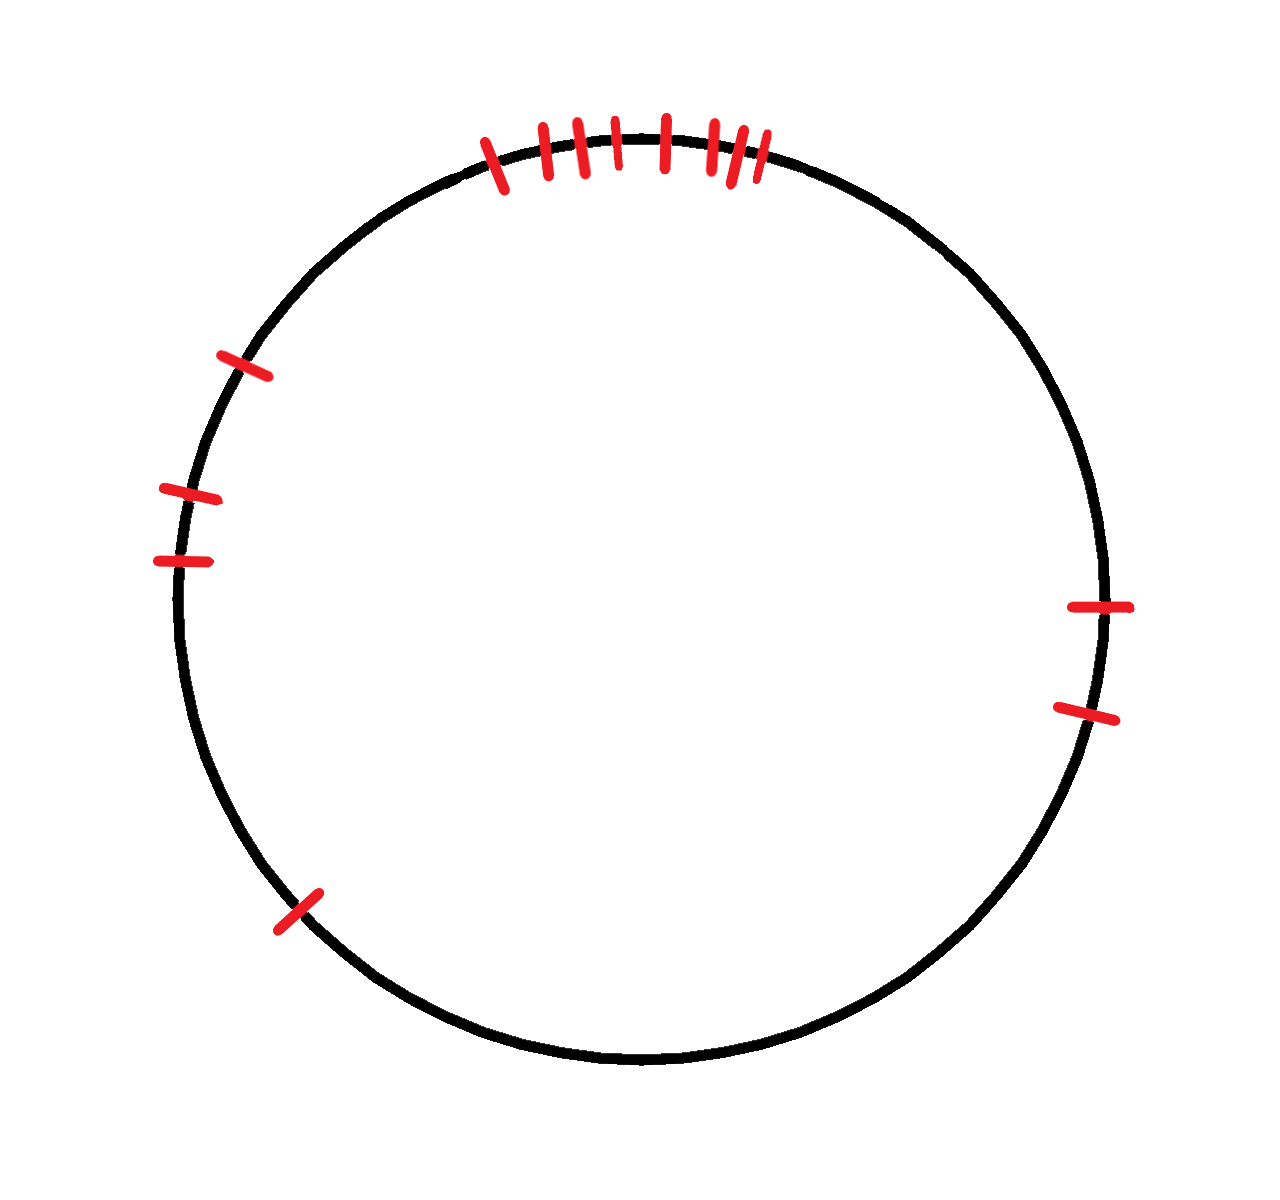
\includegraphics[width = 0.3\textwidth]{fc_fusion/7conform.png}

	\caption{A vesicle underoing full-collapse fusion.}
	\label{fig:full_collapse_fusion_multiples}
\end{figure}

\subsection{Kiss-and-Run Fusion}
Alternative to FC fusion is a process wherein the vesicle remains mostly intact in its spherical shape while the proteins flow from the vesicle onto the cell. A pore is formed at the junction of the vesicle-cell membranes, and such shape maintained over the deliver process. After a period of time the vesicle detaches and returns to the cell interior. This process is aptly named the Kiss-and-Run (KR) Fusion mode \cite{alabi2013perspectives}. An illustration is given in \autoref{fig:kiss_run_fusion_multiples}.

\begin{figure}
	\centering

	\includegraphics[width = 0.3\textwidth]{kr_fusion/3transport.png}
	\includegraphics[width = 0.3\textwidth]{kr_fusion/4dock.png}
	\includegraphics[width = 0.3\textwidth]{kr_fusion/5pore.png}

	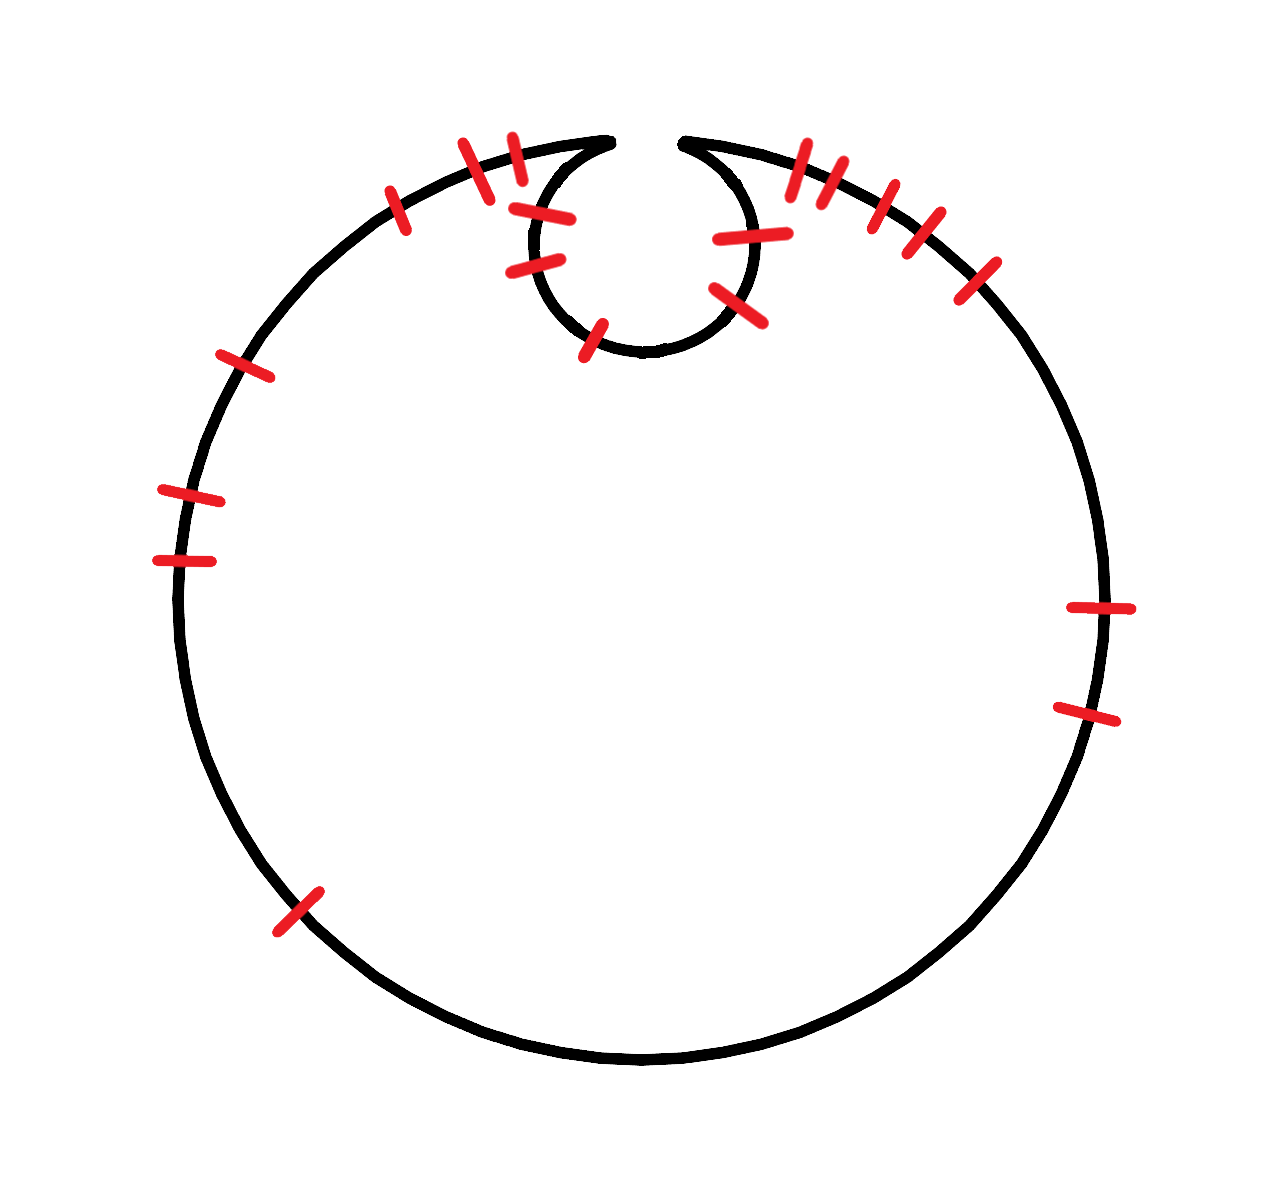
\includegraphics[width = 0.3\textwidth]{kr_fusion/6diffuse.png}
	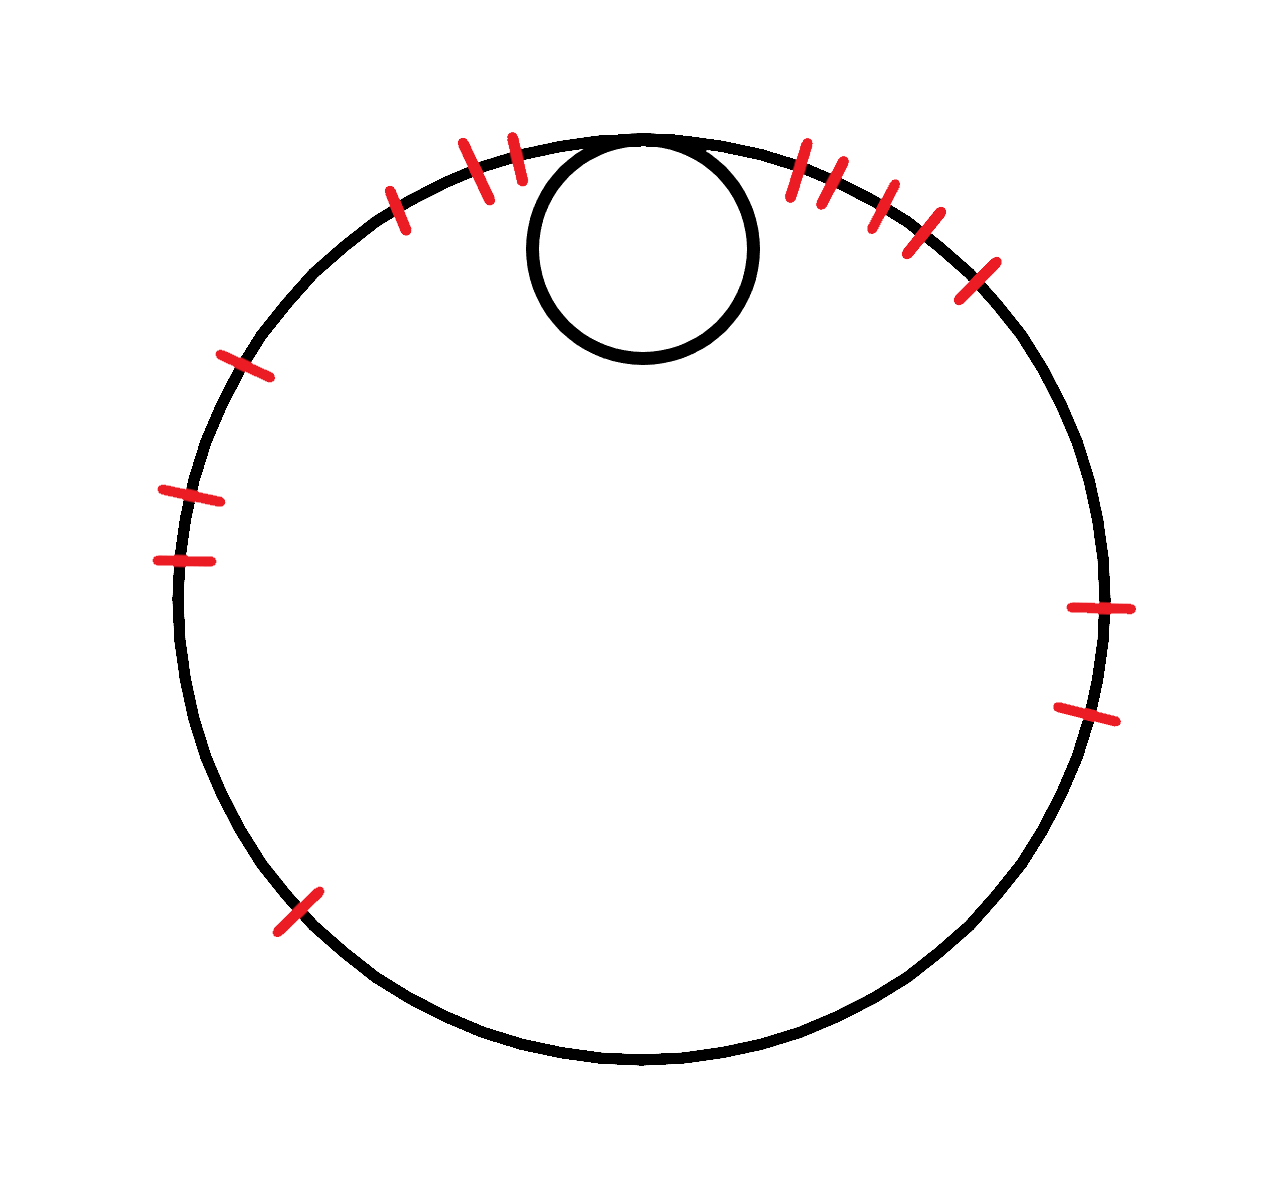
\includegraphics[width = 0.3\textwidth]{kr_fusion/7detach.png}
	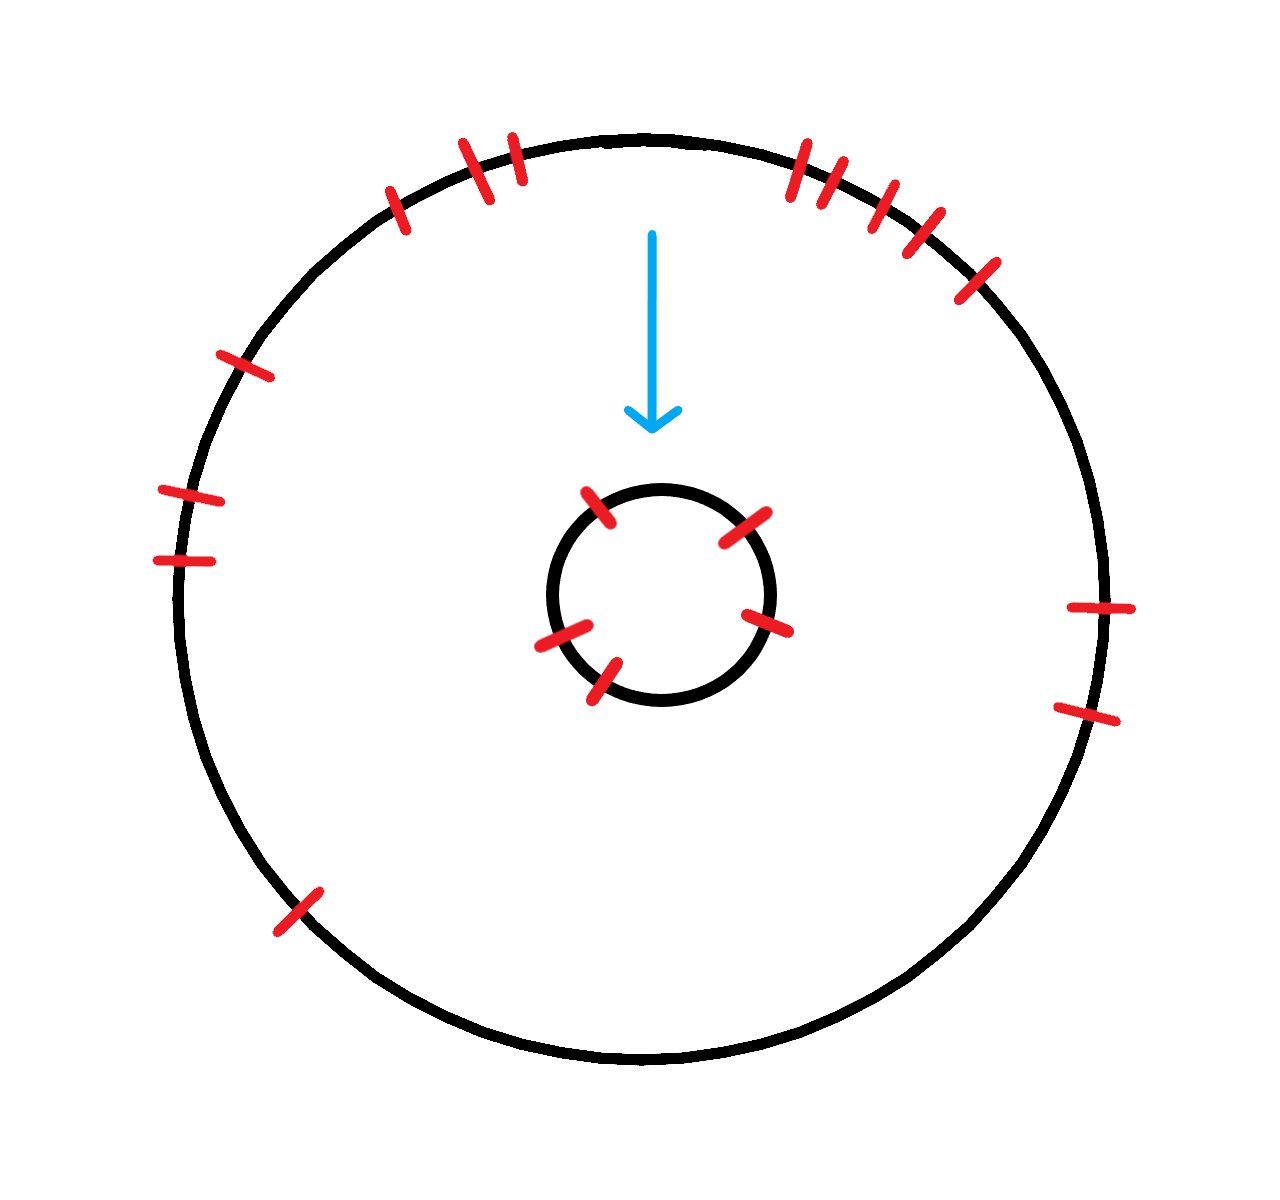
\includegraphics[width = 0.3\textwidth]{kr_fusion/8recycle.png}

	\caption{A vesicle underoing kiss-and-run fusion.}
	\label{fig:kiss_run_fusion_multiples}
\end{figure}

While KR fusion is energetically unfavourable over FC, it enables the recycling and reuse of vesicles, which can be essential in scenarios where vesicles are in short supply \cite{harata2006kiss}. Otherwise energy is expended in the re-creation of vesicles through budding off the cell membrane, or from the cell's interior\footnote{Check: can cells produce vesicles from their interior?}. Such energy usage may be more than is expended in KR fusion\footnote{Also check}.

\subsection{Fusion Pore}


\section{Diffusion}
Author note: edit: the following events/states are not alternatives.

The arrival of membrane proteins at the cell membrane from the fused vesicle can result in a local concentration spike. In some delivery contexts the following stage finds the proteins remaining clustered by the enforcement of other cell-membranous contents \cite{lillemeier2006plasma, willig2006sted}.

The energetically favourable alternative is the topic of study, wherein the proteins redistribute to equilibrate the concentration across the membrane surface [REF], as observed in [REF]. This process of diffusion is the central focus of study for this paper.

While diffusion in cells can refer to the transport of molecules between the cellular interior and exterior facilitated by vesicles and proteins [REF], this study uses the term diffusion to refer to the lateral movement of the proteins within the confines of the cellular membrane [REF].

Diffusivity is the measure of the rate of movement of a substance with time in a particular medium. The lateral diffusivity of a membrane is influenced by its composition. Thus diffusivity can vary on the vesicle and cell membranes.

\subsection{Delivery Timing}
Due to TODO, the delivery of membrane proteins via diffusion typically does not start until the vesicle is established in its fusion form.

\cite{soykan2017synaptic}.

\section{Energetics}
Vesicular fusion requires energy [REF]. The synthesis of a vesicle also costs resources and energy. Thus, kiss-and-run fusion enables resource and energy saving at the cost of maintaining the small delivery pore at the junction of the two membrane manifolds, which however requires energy. In contrast, full fusion results in the vesicle membrane incorporated into the cell membrane. This costs less energy since the membranes converge to an energetic equilibrium. However, any further protein delivery requires the synthesis of more vesicles [REF].

\chapter{Active Research}
\section{Observations}
A cell's bias toward either of the two delivery modes may indicate the underlying processes and mechanisms acting in the cell, with regards to energy expenditure and available resources. This is one motivation for tracking vesicular delivery modality.

\cite{sochacki2012imaging}.

\subsection{Electron Micrography}
Electron micrographs are of slices of frozen cells. This is because the process of obtaining the image is long compared to changes and movements within the cells. Thus, whilst high resolution of the cell such as its surface structure is obtained, there is less information regarding the cellular dynamics.

The processes of both vesicular fusion modes have been observed in electron micrography, as shown in Figure TODO.

\subsection{TIRF Microscopy}
In Total Internal Reflection Fluorescence (TIRF) Microscopy (TIRFM), or Evanescent Wave Microscopy, proteins are tagged with a fluorescent molecule. The surface to be observed is placed on a microscope coverslip and a laser beam shone on the sample, incident at an angle greater than the critical angle for the coverslip, causing total internal reflection. Not all the energy of the incident light is reflected however, and the evanescent wave, which penetrates the sample, causes the excitation of the fluorophores to depths of around 100 nm, with intensity decaying exponentially. This enables the observation of molecules around the surface of the sample [REF].

In live cell imaging, a sequence of images are recorded, producing a movie of changes occuring at the cell surface [REF].

These frames display pixelated intensity levels at the surface of the cell. An example of such a frame is shown in Figure TODO.

Experimentally, it is often easier to label the membrane embedded contents rather than the contents in the vesicle's interior, allowing experimentalists to also observe these types of fusion events.

The main feature of TIRFM observations of vesicle fusions is the brightness of the spots that appear when the vesicle fuses. An example is shown as the red line plot of the centre profile in Figure TODO. Notice the spike in brightness due to the fusion of the vesicle to the cell, when the vesicle membrane has a high concentration of vesicles relative to the local cell membrane. The subsequent decay in the intensity is due to the diffusion of the proteins from the initial spot region onto the cell membrane [REF].

\subsubsection{Frame Rate}
Overexposure of the fluoresced proteins results in bleaching [REF]. As a result, TIRFM snapshots are either of high frame rate for a short period of time, or low frame rate over a longer period of time [REF].

\subsubsection{Observation Zone}
As aforementioned, observable fluorescence decays exponentially with depth from the viewing platform [REF] which provides the advantage of limiting observations to and just below the surface of, with the disadvantage of no observation for cellular internals \cite{axelrod2001total}.

Also recorded in TIRFM are the approach and departure of vesicles via the gradual appearance of a local spot brightness in the former, and the gradual disappearance in the latter.

Furthermore, polarized light sources enable selective excitation of fluorophores, such as restriction to membranes parallel to the substrate \cite{axelrod1989total}.

\subsection{}
\cite{he2006two}.

\subsection{Stimulated Emission Depletion}
\cite{willig2006sted}.

\section{Applications}
\begin{itemize}
	\item Therapeutic drug design targeting membrane proteins.
	\item Specific membrane protein extractions via detergents.
	\item Simulations \cite{marrink2019computational} and a case of artificial replications \cite{de2006controlled}.
\end{itemize}

\part{Mathematical Model}

\chapter{Mathematical Background}
\section{Objective}
This study seeks to identify the distinguishing features of the protein dynamics associated with full fusion and kiss-and-run fusion modes. It particularly investigates whether it is theoretically possible to resolve the fusion mode from the evolution of the distribution of proteins at the cell surface.

The movement of proteins on a cell membrane is governed by diffusion. The fusion and diffusion processes are explored for the geometries involved in full fusion and kiss-and-run fusion. The membranes involved are approximated as spherical manifolds.

A classifier for experimental fusion observations is developed here. The main experimental observation is the intensity of the fusion spot, Figure TODO. For the theoretical analogue, the spot intensity is defined to be the normalized total concentration of proteins in the initial spot-region where a vesicle has fused to the cell membrane. The nomenclature is consistent with the fact that the total number of proteins in an area is proportional to the intensity of fluorescence seen in TIRF microscopy.

Due to the limited resolution of the experimental data, it is not possible to observe all the details of the dynamics at a vesicular scale. Instead, experiments track the pixelated spot intensity as a function of discrete time steps. The mathematical models have the advantage of analysis with ``infinite'' resolution in both space and time.

Of auxiliary usefulness is the intensity of the ring around the fusion spot. Both fusion modes are inticipated to have similar intensity dynamics, yet the surrounding ring is expected to have stronger distinctions. In observations, the ring intensity can distinguish between a transiting vesicle under the surface from an actual fusion event.

Also modelled is the TIRFM observation zone, wherein the fluorescence decays exponentially with depth.

\section{Existing Models}
\cite{marrink2019computational}.
\cite{jorgensen2017computer}.
\cite{risselada2020proteins}.

\section{Notation}
The standard Cartesian coordinate system in three dimensions are described using $\vec{x} = (x, y, z)$ with positive directions defined via the right-hand rule. The vertical coordinate $z$ is replaced in some modelling contexts with $\xi$ and $\ze$, which are simply vertical offsets sharing horizontal coordinates $(x, y)$.

The dimension of time is represented by the variable $t$.

Proteins are treated as infinitesimal, parameterised and treated similarly to heat. Symbols of use are $u$, $v$ and $c$ which will be defined in their respective contexts. The term concentration is used interchangeably with density.

The parameter of the flux of proteins is represented by $J$ as a scalar, or $\vec{J}$ as a vector, and is minimally but vitally explored. It's involvment is implicity in other parameters.

The rate of diffusion of proteins is termed the diffusivity, notated $D$.

Distances from the coordinate origin in spherical coordinates is denoted by $r$ as a variable, and $R$ as a constant. The respective polar angle is expressed as $\varphi$, $\phi$, and $\psi$ introduced as needed with the model derivation.

The use of angle brackets $\Angle{\bullet}$ are typically used to denote inner products in linear algebra, and integrated averages over time or another continuous parameter in physical sciences. In this paper, a definition similar to both is employed as defined in TODO.

As demonstrated in the previous paragraph, a bullet $\bullet$ is sometimes used as a placeholder for a variable or function.

The same physical parameters are explored in different micro-contexts, required either alternative use of symbol (as above with concentration and vertical coordinate) or symbol embellishment for distinction. for distinction between pre- and post-fusion parameters, a prime $\bullet'$ is used to denote post-fusion parameter. The absence of a prime however does not imply strictly pre-fusion.

The Heaviside function is used extensively in the modelling process, and is denoted $H(x)$, defined as
\begin{align*}
	H(x) &= \begin{cases}
		0 & x < 0 \\
		0.5 & x = 0 \\
		1 & x > 0
	\end{cases}
\end{align*}

$\delta_{mn}$ is the Kronecker delta,
\begin{align*}
	\delta_{mn} &= \begin{cases}
		0 & m \neq n \\
		1 & m = n
	\end{cases}
\end{align*}

Topological set theory notation is used, particularly $\overline\bullet$ to denote set closure, $\partial\bullet$ for the boundary/ies of a set, $\inf\bullet$ and $\sup\bullet$ respectively denoting the infimum and supremum (boundaries) of the set $\bullet$, and $\conv\bullet$ denoting the convex hull of the set $\bullet$. Motivation for such uses are for concise expression and this paper does not explore any rigorous topology or differential geometry.

Other set notation used are the classical symbols of $\bbR$ for the real numbers and $\bbZ$ for the integers. The strictly positive integers are denoted $\bbZ^+$ and to include zero, $\bbZ_0^+$. $\bbP$ is used to denote the set of valid integer values for an index in the derived models, $\bbP = \Brace{0, 1, 2, ..., P-1, P}$ for $P \in \bbZ^+$.

\section{Modelling Theory}
The following description is of a model built on the theory of differential equations, the finite element method, 

All scenarios analysed in this paper are axisymmetric and restricted to the surface of a sphere.

Metric units are considered consistent, and are not defined until TODO.

\chapter{Diffusion}
Protein delivery dynamics are here modelled as a scaled concentration diffusion on the surface of static membrane manifolds. Full fusion is modelled on the surface of a sphere, and kiss-and-run fusion on the surface of two truncated, connected spheres. The physical parameters involved in each model are derived from the pre-fusion cell and delivery vesicle parameters. The diffusion equation is then solved on the manifold defined by those parameters.

The membranes are modelled as static due to the diffusion of proteins not starting until the vesicle is established in its fusion form structure, see TODO.

\section{Conservation of Mass}
The diffusion model assumes no source or sink for proteins, hence a conservation of mass expressed as follows.

\begin{align*}
	\pdv{u}{t} &= -\nabla \dotproduct \vec{J}
\end{align*}

\section{Fick's First Law of Diffusion}
Fick's first law of diffusion simply states that the flux goes from high to low levels of concentration.

\begin{align*}
	\vec{J}(\vec{x}, t) &= -D(\vec{x}, t) \nabla{u(\vec{x}, t)}
\end{align*}

\section{Diffusion Equation}
The diffusion equation is obtained via equating the flux under the law of mass conservation with Fick's first law of diffusion.
\begin{align*}
	\pdv{u(\vec{x}, t)}{t} &= \nabla \dotproduct \Brack{D(\vec{x}, t)\ \nabla{u(\vec{x}, t)}}
\end{align*}

In spherical coordinates with azimuthal symmetry on the surface of a sphere,
\begin{align*}
	r^2 \sin(\varphi) \pdv{u}{t} &= \pdv{}{\varphi}\Par{D(\varphi) \sin(\varphi) \pdv{u}{\varphi}}
\end{align*}

\section{Pre-Fusion Parameters}
The fusion events in question involve the dynamics of two spherical membranes connecting to form a fused system. Preceding any contact, the physical features of the two membranes are parameterised for their spherical radius and membrane protein diffusivity. Specifically, subscripts $\bullet_v$ and $\bullet_c$ are used to denote parameters for the vesicle and cell respecitvely. The model input constants are $R_v$ and $R_c$ for the pre-fusion radii and $D_v$ and $D_c$ for the diffusivites.

The fusion events result in geometric deformities that demand the calculation of further post-fusion parameters. However the diffusivities are assumed to persist.

Though it is highly unrealistic for a vesicle to approach the size of the cell, such a scenario provides a convenient way to test the validity of the derived models.

\section{Total Concentration}
The objective output variable of interest is the intensity, otherwise termed the integration of the normalised concentration level over a specified spatial domain $\Theta$.

\begin{align*}
	\Angle{\bullet}_\Theta &= r^2 \int_\Theta \bullet \sin(\varphi)\ \dd\varphi
\end{align*}

This definition is later re-derived into a form used due to the model derivation process, given in TODO and TODO.

\section{Fusion}

For both fusion events, the following assumptions are made.

\subsection{Conservation of Surface Area}
Pre-fusion, the vesicle and cell surface areas are given as
\begin{align*}
	\SA_v &= 4\pi R_v^2 \\
	\SA_c &= 4\pi R_c^2
\end{align*}

\chapter{Full Fusion}
\section{Fusion Parameters}
The process of full fusion results in the vesicle becoming fully incorporated into the geometrical structure of a cell. This results in a post-fusion sphere, which is modelled with polar angle $\varphi \in \overline\Theta$ with $\Theta = (0, \pi)$. The vesicle becomes fused as a polar cap on the fused system. The system maintains its axisymmetry.

\subsection{Post-Fusion Radii}
Under the assumption of surface area preservation,
\begin{align*}
	\SA_\text{FC} &= \SA_v + \SA_c \\
	\Rightarrow 4\pi \R^2 &= 4\pi R_v^2 + 4\pi R_c^2 \\
	\Rightarrow \R &= \sqrt{R_v^2 + R_c^2}
\end{align*}
where the post-fusion spherical radius is denoted as $\R > 0$.

\subsection{Junction Angle}
The fused system results in the vesicle and cell membrane meeting at a location termed the junction, denoted by the polar angle as $\varphi_j$. The location of this junction is derived from the fact that the vesicle's preserved surface area occupies the fused sphere as a spherical cap.
\begin{align}
	\SA_\text{cap} &= \SA_v \nonumber \\
	\Rightarrow 2\pi \R^2 \Par{1 - \cos(\varphi_j)} &= 4\pi R_v^2 \nonumber \\
	\Rightarrow \varphi_j &= \cos^{-1}\Par{1 - \frac{2R_v^2}{\R^2}} \nonumber \\
	&= \cos^{-1}\Par{\frac{R_c^2 - R_v^2}{\R^2}} \label{eqn:FC:junction_angle}
\end{align}
for $\varphi_j \in \Theta$.

\subsection{Diffusivity}
The full fusion model assumes conservation of diffusivity, resulting in a junction consisting of a potential diffusivity transition. This is modelled as Heaviside.
\begin{align*}
	D(\varphi) &= D_v H(\varphi_j - \varphi) + D_c H(\varphi - \varphi_j)
\end{align*}

\section{Initial-and-Boundary Value Problem}
The diffusion equation applied to the full fusion model with parameters defined above provides the initial-and-boundary value problem as follows.
\begin{align*}
	\R^2 \sin(\varphi) \pdv{u(\varphi, t)}{t} &= \pdv\varphi\Par{D(\varphi) \sin(\varphi) \pdv{u(\varphi, t)}{\varphi}}
	& \varphi &\in \Theta
	& t &> 0 \\
	u(\varphi, t) &= H(\varphi_j - \varphi)
	& \varphi &\in \overline\Theta
	& t &= 0 \\
	\pdv{u(\varphi, t)}{\varphi} &= 0 & \varphi &\in \partial\Theta & t &\geq 0
\end{align*}

\section{Analytical Solution for Constant Diffusivity}
The frontier of analytical solution methods for the diffusion problem specified above involves constant diffusivity. Though deriving such a solution is of limited scope, it provides a useful validity test for the implementation.

By constant diffusivity, $D(\varphi) = D$ so
\begin{align*}
	\frac{\R^2}{D} \pdv{u(\varphi, t)}{t} &= \frac{1}{\sin(\varphi)}\pdv\varphi\Par{\sin(\varphi) \pdv{u(\varphi, t)}{\varphi}}
\end{align*}

Via the method of separation of variables for partial differential equations, we assume
\begin{align*}
	u(\varphi, t) &= \Phi(\phi) T(t)
\end{align*}
and substitution into the full fusion diffusion equation yields the pair of equations
\begin{align*}
	0 &= \dv{T(t)}{t} + \frac{\lambda D}{\R^2} T(t) \\
	0 &= \frac{1}{\sin(\varphi)} \dv{\varphi}\Par{\sin(\varphi) \dv{\Phi(\varphi)}{\varphi}} + \lambda \Phi(\varphi)
\end{align*}
with separation constant $-\lambda$. The temporal equation admits solution form
\begin{align*}
	T(t) &= \exp\Brace{\frac{-\lambda D}{\R^2} t}
\end{align*}
Let our spatial transform project to the vertical coordinate $z = \cos(\varphi)$ with $\Phi(\varphi) = Z(z)$, so
\begin{align*}
	0 &= \dv{z}\Par{\Par{1 - z^2} \dv{Z(z)}{z}} + \lambda Z(z)
\end{align*}
which admits eigenfunction solutions of the form
\begin{align*}
	Z_n(z) &= P_n(z) & n &= 0, 1, 2, ...
\end{align*}
where $P_n$ is the $n^\text{th}$ Legendre Polynomial of the first kind, with eigenvalues
\begin{align*}
	\lambda_n &= n \Par{n + 1} & n &= 0, 1, 2, ...
\end{align*}
and our solution holds the form
\begin{align*}
	u(\varphi, t) &= \sum_{n = 0}^\infty c_n P_n\Par{\cos(\varphi)} \exp\Brace{\frac{-\lambda_n D}{\R^2} t}
\end{align*}
Applying the initial condition (with vertical coordinate for clarity)\footnote{Author Note: Check validity of interchanging infinite sum with definite integral.},
\begin{align*}
	H(z - z_j) &= \sum_{n = 0}^\infty c_n P_n(z) \\
	\Rightarrow H(z - z_j) P_m(z) &= P_m(z) \sum_{n = 0}^\infty c_n P_n(z) & m &= 0, 1, 2, ... \\
	&= \sum_{n = 0}^\infty c_n P_m(z) P_n(z) & m &= 0, 1, 2, ... \\
	\Rightarrow \int_{-1}^1 H(z - z_j) P_m(z) \dd{z} &= \int_{-1}^1 \sum_{n = 0}^\infty c_n P_m(z) P_n(z) \dd{z} & m &= 0, 1, 2, ... \\
	&= \sum_{n=0}^\infty c_n \int_{-1}^1 P_m(z) P_n(z) \dd{z} & m &= 0, 1, 2, ... \\
	&= \sum_{n=0}^\infty c_n \frac{2 \delta_{mn}}{2n + 1}
\end{align*}
and for $m = 0$,
\begin{align*}
	\text{LHS} &= \int_{z_j}^1 \dd{z} \\
	&= 1 - z_j
\end{align*}
but for $m = 1, 2, 3, ...$,\footnote{Author note: reference identity}
\begin{align*}
	\text{LHS} &= \int_{-1}^1 H(z - z_j) P_m(z) \dd{z} \\
	&= \int_{z_j}^1 P_m(z) \dd{z} \\
	&= \frac{1}{2m + 1} \Brack{P_{m+1}(z) - P_{m-1}(z)}_{z_j}^1 \\
	&= \frac{P_{m+1}(z_j) - P_{m-1}(z_j)}{2m + 1}
\end{align*}
thus for $m = n$,
\begin{align*}
	c_n &= \begin{cases}
		\dfrac{1 - \cos(\phi_j)}{2} & n = 0 \\ \\
		\dfrac{P_{n+1}\Par{\cos\phi_j} - P_{n-1}\Par{\cos\phi_j}}{2} & n = 1, 2, 3, ...
	\end{cases}
\end{align*}

\section{Weak Form}
The numerical solution in prospect requires reformulation of the differential equation in weak form as follows. With $w(\varphi)$ the test function,
\begin{align*}
	\R^2 \sin(\varphi) \pdv{u(\varphi, t)}{t} &= \pdv\varphi\Par{D(\varphi) \sin(\varphi) \pdv{u(\varphi, t)}{\varphi}} \\
	\R^2 \sin(\varphi) \pdv{u(\varphi, t)}{t} w(\varphi) &= \pdv\varphi\Par{D(\varphi) \sin(\varphi) \pdv{u(\varphi, t)}{\varphi}} w(\varphi) \\
	\R^2 \int_\Theta \sin(\varphi) \pdv{u(\varphi, t)}{t} w(\varphi) \dd\varphi &= \int_\Theta \pdv\varphi\Par{D(\varphi) \sin(\varphi) \pdv{u(\varphi, t)}{\varphi}} w(\varphi) \dd\varphi \\
	\Angle{\pdv{u(\varphi, t)}{t} w(\varphi)} &= \Brack{D(\varphi) \sin(\varphi) \pdv{u(\varphi, t)}{\varphi} w(\varphi)}_\Theta
	- \int_\Theta D(\varphi) \sin(\varphi) \pdv{u(\varphi, t)}{\varphi} \dv{w(\varphi)}{\varphi} \dd\varphi \\
	\Angle{\pdv{u(\varphi, t)}{t} w(\varphi)} &= -\int_\Theta D(\varphi) \sin(\varphi) \pdv{u(\varphi, t)}{\varphi} \dv{w(\varphi)}{\varphi} \dd\varphi \\
	\Angle{\pdv{u(\varphi, t)}{t} w(\varphi)} &= - \frac{1}{2\pi \R^2} \Angle{D(\varphi) \pdv{u(\varphi, t)}{\varphi} \dv{w(\varphi)}{\varphi}}
\end{align*}
yielding the weak form
\begin{align*}
	0 &= \Angle{\pdv{u(\varphi, t)}{t} w(\varphi)} + \frac{1}{\R^2} \Angle{D(\varphi) \pdv{u(\varphi, t)}{\varphi} \dv{w(\varphi)}{\varphi}}
\end{align*}
with total concentration
\begin{align*}
	\Angle{\bullet} &= \R^2 \int_\Theta \sin(\varphi) \bullet \dd\varphi
\end{align*}

\subsection{Parameterisation by Arc Length}
By foresight of the kiss-and-run fusion modelling, we parameterize the full fusion weak form by arc length.
\begin{align*}
	\varphi &= \frac{s(\varphi)}{\R}
\end{align*}
providing the new weak form
\begin{align*}
	0 &= \Angle{\pdv{u(s, t)}{t} w(s)} + \Angle{D(s) \pdv{u(s, t)}{s} \dv{w(s)}{s}}
\end{align*}
with
\begin{align*}
	\omega(s) &= \frac{s}{\R} \\
	\Angle\bullet &= 2\pi \R \int_\Omega \sin\Par{\omega(s)} \bullet \dd{s}
\end{align*}

\section{Steady State Solution}
The expected steady state is easily computed since the total concentration becomes evenly spread over the domain.
\begin{align*}
	\lim_{t \to \infty} u(s, t) &= \frac{\SA_\text{cap}}{\SA_\text{FC}} \\
	&= \frac{\SA_v}{\SA_v + \SA_c} \\
	&= \frac{4\pi R_v^2}{4\pi \Par{R_v^2 + R_c^2}} \\
	&= \frac{R_v^2}{\R^2}
\end{align*}
In minimizing the expression further using \eqref{eqn:FC:junction_angle},
\begin{align*}
	\lim_{t \to \infty} u(s, t) &= \frac{R_v^2}{\R^2} \\
	&= \frac{1 - \cos(\varphi_j)}{2}
\end{align*}

\chapter{Kiss-and-Run Fusion}
\section{Fusion Parameters}
The process of kiss-and-run fusion results in the vesicle mostly retaining its spherical shape. The cell similarly retains its shape, but both membranes attain an opening or pore of circular geometry with radius denoted $R_j$. The fused system is assigned two coordinate systems, one for each membrane with polar angles $\phi \in \Omega_v$ for the vesicle and $\psi = \Omega_c$ on the cell. The respective domains are derived as following, such that $\Abs{\Omega_v} = \phi_v$ and $\Abs{\Omega_c} = \psi_c$.

\subsection{Post-Fusion Radii}
Under the assumption of surface area preservation, the vesicle undergoes perforation resulting in a polar cap domain void.
\begin{align*}
	\SA'_v &= \SA_v \\
	\Rightarrow 2\pi \Rv^2 \int_0^{\phi_v} \sin\phi \dd{\phi} &= 4\pi R_v^2 \\
	\Rightarrow \Rv^2 \Par{1 - \cos\phi_v} &= 2 R_v^2
\end{align*}
Also note from the trigonometry,
\begin{align*}
	\cos(\phi_v) &= \frac{-\sqrt{\Rv^2 - R_j^2}}{\Rv}
\end{align*}
where the negative root arises from our choice of $\phi_v$ in the second quadrant. Thus,
\begin{align*}
	\Rv^2 \Par{1 - \cos\phi_v} &= 2 R_v^2 \\
	\Rightarrow \Rv^2 \Par{1 + \frac{\sqrt{\Rv^2 - R_j^2}}{\Rv}} &= 2 R_v^2 \\
	\Rightarrow \Rv^2 + \Rv\sqrt{\Rv^2 - R_j^2} &= 2 R_v^2 \\
	\Rightarrow \sqrt{\Rv^2 - R_j^2} &= \frac{2 R_v^2 - \Rv^2}{\Rv} \\
	\Rightarrow \Rv^2 - R_j^2 &= \frac{\Par{2 R_v^2 - \Rv^2}^2}{\Rv^2} \\
	\Rightarrow \Rv^4 - R_j^2 \Rv^2 &= 4R_v^4 - 4R_v^2\Rv^2 + \Rv^4 \\
	\Rightarrow -R_j^2 \Rv^2 &= 4R_v^4 - 4R_v^2\Rv^2 \\
	\Rightarrow \Rv^2\Par{4R_v^2 - R_j^2} &= 4R_v^4 \\
	\Rightarrow \Rv^2 &= \frac{4R_v^4}{4R_v^2 - R_j^2} \\
	\Rightarrow \Rv &= \frac{2R_v^2}{\sqrt{4R_v^2 - R_j^2}}
\end{align*}

By the same reasoning,
\begin{align*}
	\Rc &= \frac{2R_c^2}{\sqrt{4R_c^2 - R_j^2}}
\end{align*}

\subsection{Junction Angles}
By the geometry,
\begin{align*}
	\phi_v &= \pi - \sin^{-1}\Par{\frac{R_j}{\Rv}} \\
	\psi_c &= \pi - \sin^{-1}\Par{\frac{R_j}{\Rc}}
\end{align*}

\section{Initial-and-Boundary Value Problem}
The domain of our differential equation is of two connected truncated spheres, connected at their truncations.
\begin{align*}
	\Omega_v &= (0, \phi_v) \\
	\Omega_c &= (\pi - \psi_c, \pi)
\end{align*}

The initial-and-boundary value problem is of a connection of two systems such that
\begin{align*}
	\Rv^2 \sin(\phi) \pdv{v(\phi, t)}{t} &= D_v \pdv\phi \Par{\sin(\phi) \pdv{v(\phi, t)}{\phi}}
	& \phi &\in \Omega_v
	& t &\geq 0 \\
	\Rc^2 \sin(\psi) \pdv{c(\psi, t)}{t} &= D_c \pdv\psi \Par{\sin(\psi) \pdv{c(\psi, t)}{\psi}}
	& \psi &\in \Omega_c
	& t &\geq 0
\end{align*}

Initially,
\begin{align*}
	v(\phi, t) &= 1 & \phi &\in \Omega_v & & & t &= 0 \\
	c(\psi, t) &= 0 & & & \psi &\in \Omega_c & t &= 0
\end{align*}

At the junction,
\begin{align*}
	v(\phi, t) &= c(\psi, t)
	& \phi &= \sup\Omega_v
	& \psi &= \inf\Omega_c
	& t &\geq 0 \\
	\frac{D_v}{\Rv} \pdv{v(\phi, t)}{\phi} &= \frac{D_c}{\Rc} \pdv{c(\psi, t)}{\psi}
	& \phi &= \sup\Omega_v
	& \psi &= \inf\Omega_c
	& t &\geq 0
\end{align*}

And initially at the junction,
\begin{align*}
	v(\phi, t) &= c(\psi, t) = 0.5 & \phi &\in \Omega_v & \psi &\in \Omega_c & t &\in \bbR_0^+
\end{align*}
imitating a Heaviside transition.

\section{Weak Form}
The weak form is developed with $f(\phi)$ and $g(\psi)$ as test functions.

On the vesicle,
\begin{align*}
	\Rv^2 \sin(\phi) \pdv{v(\phi, t)}{t} &= D_v \pdv\phi \Par{\sin(\phi) \pdv{v(\phi, t)}{\phi}} \\
	\Rv^2 \sin(\phi) \pdv{v(\phi, t)}{t} f(\phi) &= D_v \pdv\phi \Par{\sin(\phi) \pdv{v(\phi, t)}{\phi}} f(\phi) \\
	\Rv^2 \int_{\Omega_v} \sin(\phi) \pdv{v(\phi, t)}{t} f(\phi)\ \dd\phi &= D_v \int_{\Omega_v} \pdv\phi \Par{\sin(\phi) \pdv{v(\phi, t)}{\phi}} f(\phi)\ \dd\phi \\
	\Rv^2 \int_{\Omega_v} \sin(\phi) \pdv{v(\phi, t)}{t} f(\phi)\ \dd\phi &= D_v \int_{\Omega_v} \pdv\phi \Par{\sin(\phi) \pdv{v(\phi, t)}{\phi}} f(\phi)\ \dd\phi \\
	\Angle{\pdv{v(\phi, t)}{t} f(\phi)}_v &= D_v \Par{\Brack{\sin(\phi) \pdv{v(\phi, t)}{\phi} f(\phi)}_{\Omega_v} - \int_{\Omega_v} \sin(\phi) \pdv{v(\phi, t)}{\phi} \pdv{f(\phi)}{\phi}\ \dd\phi} \\
	\Angle{\pdv{v(\phi, t)}{t} f(\phi)}_v &= D_v \Par{\Brack{\sin(\phi_v) \pdv{v(\phi_v, t)}{\phi} f(\phi_v) - 0} - \frac{1}{2\pi \Rv^2} \Angle{\pdv{v(\phi, t)}{\phi} \pdv{f(\phi)}{\phi}}} \\
	\Angle{\pdv{v(\phi, t)}{t} f(\phi)}_v &= D_v \Par{\sin(\phi_v) \pdv{v(\phi_v, t)}{\phi} f(\phi_v) - \frac{1}{2\pi \Rv^2} \Angle{\pdv{v(\phi, t)}{\phi} \pdv{f(\phi)}{\phi}}}
\end{align*}

On the cell,
\begin{align*}
	\Rc^2 \sin(\psi) \pdv{c(\psi, t)}{t} &= D_c \pdv\psi \Par{\sin(\psi) \pdv{c(\psi, t)}{\psi}} \\
	\Angle{\pdv{c(\psi, t)}{t} g(\psi)}_c &= D_c \Par{\Brack{\sin(\psi) \pdv{c(\psi, t)}{\psi} g(\psi)}_{\Omega_v} - \int_{\Omega_v} \sin(\psi) \pdv{c(\psi, t)}{\psi} \pdv{g(\psi)}{\psi}\ \dd\psi} \\
	\Angle{\pdv{c(\psi, t)}{t} g(\psi)}_c &= D_c \Par{\Brack{0 - \sin(\pi - \psi_v) \pdv{c(\pi - \psi_v, t)}{\psi} g(\pi - \psi_v)} - \frac{1}{2\pi \Rc^2} \Angle{\pdv{c(\psi, t)}{\psi} \pdv{g(\psi)}{\psi}}} \\
	\Angle{\pdv{c(\psi, t)}{t} g(\psi)}_c &= -D_c \Par{\sin(\pi - \psi_v) \pdv{c(\pi - \psi_v, t)}{\psi} g(\pi - \psi_v) + \frac{1}{2\pi \Rc^2} \Angle{\pdv{c(\psi, t)}{\psi} \pdv{g(\psi)}{\psi}}}
\end{align*}

Adding the two expressions,
\begin{align*}
	& \Angle{\pdv{v(\phi, t)}{t} f(\phi)}_v + \Angle{\pdv{c(\psi, t)}{t} g(\psi)}_c \\
	& \quad= D_v \sin(\phi_v) \pdv{v(\phi_v, t)}{\phi} f(\phi_v) - D_c \sin(\pi - \psi_v) \pdv{c(\pi - \psi_v, t)}{\psi} g(\pi - \psi_v) \\
	& \qquad- \Par{\frac{D_v}{\Rv^2} \Angle{\pdv{v(\phi, t)}{\phi} \pdv{f(\phi)}{\phi}} + \frac{D_c}{\Rc^2} \Angle{\pdv{c(\psi, t)}{\psi} \pdv{g(\psi)}{\psi}}}
\end{align*}
then substituting the membrane angle sizes
\begin{align*}
	& \Par{\Angle{\pdv{v(\phi, t)}{t} f(\phi)}_v + \Angle{\pdv{c(\psi, t)}{t} g(\psi)}_c} \\
	& \quad= D_v \frac{R_j}{\Rv} \pdv{v(\phi_v, t)}{\phi} f(\phi_v) - D_c \frac{R_j}{\Rc} \pdv{c(\pi - \psi_v, t)}{\psi} g(\pi - \psi_v) \\
	& \qquad- \Par{\frac{D_v}{\Rv^2} \Angle{\pdv{v(\phi, t)}{\phi} \pdv{f(\phi)}{\phi}} + \frac{D_c}{\Rc^2} \Angle{\pdv{c(\psi, t)}{\psi} \pdv{g(\psi)}{\psi}}}
\end{align*}

Select $f(\phi)$ and $g(\psi)$ such that
\begin{align*}
	f(\phi_v) &= g(\pi - \psi_c).
\end{align*}
so
\begin{align*}
	0 &= \Angle{\pdv{v(\phi, t)}{t} f(\phi)}_v + \Angle{\pdv{c(\psi, t)}{t} g(\psi)}_c \\
	&\quad+ \frac{D_v}{\Rv^2} \Angle{\pdv{v(\phi, t)}{\phi} \pdv{f(\phi)}{\phi}} + \frac{D_c}{\Rc^2} \Angle{\pdv{c(\psi, t)}{\psi} \pdv{g(\psi)}{\psi}}
\end{align*}

Define arc-length transformation such that
\begin{align*}
	s_j &= \Rv \phi_v \\
	s_P &= s_j + \Rc \psi_c \\
	s &= \begin{cases}
		\Rv \phi & \phi \in \Omega_v \\
		s_j + \Rc \Par{\psi + \psi_c - \pi} & \psi \in \Omega_c
	\end{cases}
\end{align*}
so inverse transformations are
\begin{align*}
	\Gamma_v &= (0, s_j) \\
	\Gamma_c &= (s_j, s_P) \\
	\Omega &= \conv\Par{\Gamma_v \cup \Gamma_c} \\
	\phi(s) &= \frac{s}{\Rv} \\
	\psi(s) &= \frac{s - s_j}{\Rc} + \pi - \psi_c \\\
	\omega(s) &= \begin{cases}
		\phi(s) & s \in \Gamma_v \\
		\psi(s) & s \in \Gamma_c
	\end{cases}
\end{align*}
and define $u(s, t)$ such that
\begin{align*}
	u(s, t) &= \begin{cases}
		v(\phi(s), t) & s \in \Gamma_v \\
		c(\psi(s), t) & s \in \Gamma_c
	\end{cases}
\end{align*}
so derivatives become
\begin{align*}
	\dd\phi &= \frac{1}{\Rv} \dd{s} \\
	\dd\psi &= \frac{1}{\Rc} \dd{s} \\
	\pdv{v(\phi, t)}{\phi} &= \Rv \pdv{u(s, t)}{s} \\
	\pdv{c(\psi, t)}{\psi} &= \Rc \pdv{u(s, t)}{s}
\end{align*}
and define
\begin{align*}
	w(s) &= \begin{cases}
		f(\phi(s), t) & s \in \Gamma_v \\
		g(\psi(s), t) & s \in \Gamma_c
	\end{cases}
\end{align*}
so our weak form becomes
\begin{align*}
	0 &= \Angle{\pdv{v(\phi, t)}{t} f(\phi)}_v
	+ \Angle{\pdv{c(\psi, t)}{t} g(\psi)}_c \\
	&\quad+ \frac{D_v}{\Rv^2} \Angle{\pdv{v(\phi, t)}{\phi} \pdv{f(\phi)}{\phi}}
	+ \frac{D_c}{\Rc^2} \Angle{\pdv{c(\psi, t)}{\psi} \pdv{g(\psi)}{\psi}} \\
	0 &= \Rv^2 \int_{\Omega_v} \sin(\phi) \pdv{v(\phi, t)}{t} f(\phi) \dd\phi
	+ \Rc^2 \int_{\Omega_c} \sin(\psi) \pdv{c(\psi, t)}{t} g(\psi) \dd\psi \\
	&\quad+ D_v \int_{\Omega_v} \sin(\phi) \pdv{v(\phi, t)}{\phi} \pdv{f(\phi)}{\phi} \dd\phi
	+ D_c \int_{\Omega_c} \sin(\psi) \pdv{c(\psi, t)}{\psi} \pdv{g(\psi)}{\psi} \dd\psi \\
	0 &= \Rv \int_{\Gamma_v} \sin\Par{\phi(s)} \pdv{u(s, t)}{t} w(s) \dd{s}
	+ \Rc \int_{\Gamma_c} \sin\Par{\psi(s)} \pdv{u(s, t)}{t} w(s) \dd{s} \\
	&\quad+ D_v \int_{\Gamma_v} \sin\Par{\phi(s)} \pdv{u(s, t)}{s} \dv{w(s)}{s} \dd{s} + D_c \int_{\Gamma_c} \sin\Par{\psi(s)} \pdv{u(s, t)}{s} \dv{w(s)}{s} \dd{s} \\
	0 &= \int_\Omega \sin\Par{\omega(s)} \R(s) \pdv{u(s, t)}{t} w(s) + \int_\Omega \sin\Par{\omega(s)} D(s) \pdv{u(s, t)}{s} \dv{w(s)}{s} \dd{s}
\end{align*}
yielding our weak form in arc-length
\begin{align*}
	0 &= \Angle{\pdv{u(s, t)}{t} w(s)} + \Angle{\frac{D(s)}{\R(s)} \pdv{u(s, t)}{s} \dv{w(s)}{s}}
\end{align*}
with
\begin{align*}
	\R(s) &= \begin{cases}
		\Rv & s \in \Gamma_v \\
		\Rc & s \in \Gamma_c
	\end{cases} \\
	\Angle{\bullet} &= \int \R(s) \sin\Par{\omega(s)} \bullet \dd{s}
\end{align*}

\section{Steady State Solution}
The KR steady state solution is computed via the geometry.
\begin{align*}
	\lim_{t \to \infty} u(s, t) &= \frac{\SA'_v}{\SA_\text{KR}} \\
	&= \frac{\SA'_v}{\SA'_v + \SA'_c}
\end{align*}
where
\begin{align*}
	\SA'_v &= 2\pi \Rv^2 \int_0^{\phi_v} \sin(\phi) \dd{\phi} \\
	&= 2\pi \Rv^2 \Brack{\cos(\phi)}^0_{\phi_v} \\
	&= 2\pi \Rv^2 \Par{1 - \cos(\phi_v)}
\end{align*}
and similarly
\begin{align*}
	\SA'_c &= 2\pi \Rc^2\Par{1 - \cos(\psi_c)}
\end{align*}
so
\begin{align*}
	\lim_{t \to \infty} u(s, t) &= \frac{\Rv^2 \Par{1 - \cos(\phi_v)}}{
		\Rv^2 \Par{1 - \cos(\phi_v)}
		+ \Rc^2 \Par{1 - \cos(\psi_c)}
	}
\end{align*}

\chapter{Finite Element Method}
The rigour of approximating the weak form's solution via projection onto a space of square-integrable piecewise-linear functions is not explicitly explored here. However, the theory that follows is taken from such. It will be stated however that the definition of the angle bracket operator operating on a function $\bullet$ is inspired from the inner product defined on the function space operating on $\bullet$ with one. That is,
\begin{align*}
	\Angle{\bullet} &= \Angle{\bullet, 1}
\end{align*}

The finite element method expressed generically for the fusion modes of full and kiss-and-run takes a weak formulation
\begin{align*}
	0 &= \Angle{\pdv{u(s, t)}{t} w(s)} + \Angle{\frac{D(s)}{R(s)} \pdv{u(s, t)}{s} \dv{w(s)}{s}}
\end{align*}
with
\begin{align*}
	\Angle{\bullet} &= \int_\Omega R(s) \sin\Par{\omega(s)} \bullet \dd{s}
\end{align*}
for $\Omega$, $s$, $D(s)$, $R(s)$, and $\omega(s)$ defined by the fusion mode model.

\section{Conservation of Mathematical Principles}
By the involvedness of the derivation and for the testing of implementation, the developed model is investigated for validity through application of the first principles it is derived from.

\subsection{Stability and Conservation of Mass}
The finite element method is unconditionally stable for this problem. To see this, note that the weak form given above is valid for arbitrary $w$. Choosing $w = 1$,
\begin{align*}
	0 &= \Angle{\pdv{u(s, t)}{t}} = \pdv{t} \Angle{u(s, t)}
\end{align*}
which is also a statement of conservation. This is to say, the total concentration of proteins is preserved for all time.

In function space theory, this relationship would be expressed with the $\mathcal{L}^1$ norm.

\subsection{}
Another essential feature of the model must be that TODO.

To see this, let $w = u(s, t)$ be time-dependent. Note that in the algebra and calculus manipulations in the derivations, the test functions were never subjected to the time derivative\footnote{Author note: check!}.
\begin{align*}
	0 &= \Angle{u(s)\pdv{u(s, t)}{t}} + \Angle{\frac{D(s)}{R(s)} \Par{\pdv{u(s, t)}{s}}^2} \\
	&= \Angle{\frac{1}{2} \pdv{t}\Par{u^2(s, t)}} + \Angle{\frac{D(s)}{R(s)} \Par{\pdv{u(s, t)}{s}}^2} \\
	&= \frac{1}{2} \pdv{t} \Angle{u^2(s, t)} + \Angle{\frac{D(s)}{R(s)} \Par{\pdv{u(s, t)}{s}}^2} \\
	\Rightarrow \pdv{t} \Angle{u^2(s, t)} &= -2 \Angle{\frac{D(s)}{R(s)} \Par{\pdv{u(s, t)}{s}}^2}
\end{align*}
where the $\Angle\bullet$ on the RHS is always positive, thus any change of concentration level over time is TODO.

In function space theory, this relationship would be expressed with the $\mathcal{L}^2$ norm.

\section{Spatial Discretisation}
Select positive integers $p_j$ and $P$ such that
\begin{align*}
	p_j < P
\end{align*}

Define
\begin{align*}
	\bbP &= \Brace{0, 1, 2, ..., P}
\end{align*}

Select values $s_p$ for $p \in \bbP$ such that
\begin{align*}
	0 = s_0 < s_1 < \cdots s_{p_j - 1} < s_{p_j} = s_j < s_{p_j + 1} < \cdots < s_{P - 1} < s_P
\end{align*}

Define their spacing,
\begin{align*}
	h_p &= s_p - s_{p-1} & s \in \bbP^+
\end{align*}

Define hat functions such that
\begin{align*}
	\Lambda_p(s) &= \begin{cases}
		1 & s = s_p \\
		\dfrac{s - s_{p-1}}{h_p} & s \in (s_{p-1}, s_p) \\
		\dfrac{s_{p+1} - s}{h_{p+1}} & s \in (s_p, s_{p+1}) \\
		0 & \text{otherwise}
	\end{cases}
\end{align*}

Transform the weak form into a system of equations by selecting
\begin{align*}
	w(s) &= \Lambda_p(s) & p &\in \bbP
\end{align*}
so
\begin{align*}
	0 &= \Angle{\pdv{u(s, t)}{t} \Lambda_p(s)} + \Angle{\frac{D(s)}{R(s)} \pdv{u(s, t)}{s} \pdv{\Lambda_p(s)}{s}} & p &\in \bbP
\end{align*}

Project the solution $u(s, t)$ onto the space of piecewise-linear functions defined on the discrete grid $s_p$, and define this projection as
\begin{align*}
	u_h(s, t) &= \sum_{q = 0}^P U_q(t) \Lambda_q(s)
\end{align*}
and impose this by substitution so
\begin{align*}
	0 &= \pdv{U_q(t)}{t} \Angle{\Lambda_q(s) \Lambda_p(s)} + U_q(t) \Angle{\frac{D(s)}{R(s)} \pdv{\Lambda_q(s)}{s} \pdv{\Lambda_p(s)}{s}}
\end{align*}
in Einstein notation for clarity.

Define
\begin{align*}
	\Vec{U}(t) &= \Brack{U_0(t)\ U_1(t)\ \cdots\ U_P(t)}^\text{T} \\
	\Brack{M}_{pq} &= \Angle{\Lambda_q(s) \Lambda_p(s)} \\
	\Brack{S}_{pq} &= \Angle{\frac{D(s)}{R(s)} \pdv{\Lambda_q(s)}{s} \pdv{\Lambda_p(s)}{s}}
\end{align*}
so we have our system
\begin{align*}
	0 &= M \dv{\vec{U}(t)}{t} + S \vec{U}(t)
\end{align*}
with mass matrix $M$ and stiffness matrix $S$.

\subsection{Taming Discontinuity}
A Heaviside transition of parameter values is located at the junction in both fusion modes. An optimal selection of spatial grid spacing minimizes the possibility of violating the law of conservation. This motivates placing a large concentration of points around the junction point. The junction itself must also be a grid point.

We apply cubic spacing on the vesicle and cell domains separately.

The vesicular gridding must satisfy
\begin{align*}
	s_0 &= 0
	s_{p_j} &= s_j
\end{align*}
and be concave down, which leads to
\begin{align*}
	s_p &= s_j \Par{1 - \Par{1 - \frac{p}{p_j}}^3}
\end{align*}

The cellular gridding similarly must satisfy
\begin{align*}
	s_{p_j} &= s_j \\
	s_P &= s_P
\end{align*}
and must be concave up, leading to
\begin{align*}
	s_p &= s_j + \Par{s_P - s_j} \Par{\frac{p - p_j}{P - p_j}}^3
\end{align*}

\section{Temporal Discretisation}
Due to stiffness, we select a backward Euler dynamic timestepping scheme. Define
\begin{align*}
	0 &= t_0 < t_1 < \cdots \\
	\vec{U}^n &= \vec{U}(t_n) & n &\in \bbZ_0^+
\end{align*}
so
\begin{align*}
	0 &= M \frac{\vec{U}^n - \vec{U}^{n - 1}}{\Delta{t}_n} + S \vec{U}^n \\
	0 &= M \Par{\vec{U}^n - \vec{U}^{n - 1}} + \Delta{t}_n S \vec{U}^n \\
	0 &= \Par{M + \Delta{t}_n S} \vec{U}^n - M \vec{U}^{n-1}
\end{align*}
yielding the matrix equation
\begin{align*}
	\Par{M + \Delta{t}_n S} \vec{U}^n &= M \vec{U}^{n-1}
\end{align*}

Due to accuracy needing small $h_p$, Simpson's Rule with two subintervals is used to evaluate the integral for the mass matrix to avoid machine rounding errors via division by small $h_p$ values.
\begin{align*}
	\int_a^b f(x) \dd{x} &\approx \frac{b - a}{6} \Brack{f(a) + 4 f\Par{\frac{a + b}{2}} + f(b)}
\end{align*}

Additionally, note the diagonalism, i.e.
\begin{align*}
	\Brack{M}_{pq} &= \Brack{M}_{qp} \\
	\Brack{S}_{pq} &= \Brack{S}_{qp}
\end{align*}
thus, WLOG we calculate
\begin{align*}
	& \Brack{M}_{pp}, \Brack{S}_{pp} & p &\in \bbP \tag{diagonal} \\
	& \Brack{M}_{p-1, p}, \Brack{S}_{p-1, p} & p &\in \bbP^+ \tag{off-diagonal}
\end{align*}
For clarity, define
\begin{align*}
	\bbP_- &= \Brace{0, ..., P-1} \\
	\bbP_+ &= \Brace{1, ..., P} \\
	\R(s) &= R(s) \sin\Par{\omega(s)} \\
	\D(s) &= D(s) \sin\Par{\omega(s)}
\end{align*}

\section{Mass Matrix}
For the main diagonal,
\begin{align*}
	\Brack{M}_{pp} &= \Angle{\Lambda_p^2(s)} \\
	&= \int_\Omega \R(s) \Lambda_p^2(s) \dd{s} \\
	&= I_{\bbP_+}(p) \int_{s_{p-1}}^{s_p} \R(s) \frac{s - s_{p-1}}{h_p} \dd{s} + I_{\bbP_-}(p) \int_{s_p}^{s_{p+1}} \R(s) \frac{s_{p+1} - s}{h_{p+1}} \dd{s}
\end{align*}
where the first integral is
\begin{align*}
	& \int_{s_{p-1}}^{s_p} \R(s) \frac{s - s_{p-1}}{h_p} \dd{s} \\
	&\quad = \frac{1}{h_p} \int_{s_{p-1}}^{s_p} \R(s) \Par{s - s_{p-1}} \dd{s} \\
	&\quad \approx \frac{1}{6} \Brack{
		\R(s_p) h_p
		+ 4 \R(s_{p-\nf12}) \Par{\frac{s_{p-1} + s_p}{2} - s_{p-1}}
	} \\
	&\quad = \frac{1}{6} \Brack{
		\R(s_p) h_p + 2 \R(s_{p-\nf12}) h_p
	}
\end{align*}
and the second integral is
\begin{align*}
	& \int_{s_p}^{s_{p+1}} \R(s) \frac{s_{p+1} - s}{h_{p+1}} \dd{s} \\
	&\quad = \frac{1}{h_p} \int_{s_p}^{s_{p+1}} \R(s) \Par{s_{p+1} - s} \dd{s} \\
	&\quad \approx \frac{1}{6} \Brack{
		\R(s_p) h_{p+1}
		+ 4 \R(s_{p+\nf12}) \Par{s_{p+1} - \frac{s_p + s_{p+1}}{2}}
	} \\
	&\quad = \frac{1}{6} \Brack{
		\R(s_p) h_{p+1} + 2 \R(s_{p+\nf12} h_{p+1})
	}
\end{align*}
so
\begin{align*}
	\Brack{M}_{pp} &\approx \frac{1}{6} \Par{I_{\bbP_+}(p) h_p \Brack{
		\R(s_p) + 2 \R(s_{p-\nf12})
	} + I_{\bbP_-}(p) h_{p+1} \Brack{
		\R(s_p) + 2 \R(s_{p+\nf12} )
	}}
\end{align*}
For the off-diagonals,
\begin{align*}
	\Brack{M}_{p-1, p} &= \Angle{\Lambda_{p-1}(s) \Lambda_p(s)} \\
	&= \int_\Omega \R(s) \Lambda_{p-1}(s) \Lambda_p(s) \dd{s} \\
	&= \frac{1}{h_p^2} \int_{s_{p-1}}^{s_p} \R(s) \Par{s_p - s} \Par{s - s_{p-1}} \dd{s} \\
	&\approx \frac{1}{6h_p} \Brack{
		4 \R(s_{p-\nf12}) \Par{s_p - \frac{s_{p-1} + s_p}{2}} \Par{\frac{s_{p-1} + s_p}{2} - s_{p-1}}
	}
\end{align*}
yielding
\begin{align*}
	\Brack{M}_{p-1, p} &\approx \frac{h_p}{6} \R(s_{p-\nf12})
\end{align*}

\section{Stiffness Matrix}
For the main diagonal,
\begin{align*}
	\Brack{S}_{pp} &= \Angle{\frac{D(s)}{R(s)} \Par{\pdv{\Lambda_p(s)}{s}}^2} \\
	&= \int_\Omega \D(s) \Par{\pdv{\Lambda_p(s)}{s}}^2 \dd{s} \\
	&= I_{\bbP_+}(p) \int_{s_{p-1}}^{s_p} \D(s) \frac{1}{h_p^2} \dd{s} + I_{\bbP_-}(p) \int_{s_p}^{s_{p+1}} \D(s) \frac{1}{h_{p+1}^2} \dd{s} \\
	&= \frac{I_{\bbP_+}(p)}{h_p^2} \int_{s_{p-1}}^{s_p} \D(s) \dd{s} + \frac{I_{\bbP_-}(p)}{h_{p+1}^2} \int_{s_p}^{s_{p+1}} \D(s) \dd{s}
\end{align*}
and the off diagonals,
\begin{align*}
	\Brack{S}_{p-1, p} &= \Angle{\frac{D(s)}{R(s)} \pdv{\Lambda_{p-1}(s)}{s} \pdv{\Lambda_p(s)}{s}} \\
	&= \int_\Omega \D(s) \pdv{\Lambda_{p-1}(s)}{s} \pdv{\Lambda_p(s)}{s} \dd{s} \\
	&= \int_{s_{p-1}}^{s_p} \D(s) \frac{-1}{h_p^2} \dd{s} \\
	&= \frac{-1}{h_p^2} \int_{s_{p-1}}^{s_p} \D(s) \dd{s}
\end{align*}

\chapter{Evanescent Wave Microscopy Model}
The final component of the intended  model is incorporation of parameters involved in TIRF Microscopy which limit the resolution of observations for fusion and diffusion dynamics in space and time.

The FC and KR fusion modes are compared in the same coordinate system, which will require a differing vertical coordinate for each full/truncated spherical system. Let $\zeta_\FC$, $\zeta_\KRv$, and $\zeta_\KRc$ represent vertical axes for the FC, KR vesicle, and KR cell respectively, such that their origins are located at the highest point of the system, and point positive with viewing depth. Such is illustrated in Figure TODO.
\begin{align*}
	\zeta_\FC &= \R - z \\
	\zeta_\KRv &= z - \Rv \cos(\pi - \phi_v) \\
	\zeta_\KRc &= \Rc \cos(\pi - \psi_c) - z
\end{align*}
The range for non-zero values are
\begin{align*}
	\zeta_\FC &\in \Gamma_\FC = \Par{0, 2\R} \\
	\zeta_\KRv &\in \Gamma_\KRv = \Par{0, \Rv \Par{1 + \cos(\pi - \phi_v)}} \\
	\zeta_\KRc &\in \Gamma_\KRc = \Par{0, \Rc \Par{1 + \cos(\pi - \psi_c)}}
\end{align*}
Additionally, we define the upper and lower regions of each domain.
\begin{align*}
	\Gamma_\FC^- &= \Par{0, \R}
	& \Gamma_\FC^+ &= \Par{\R, 2\R} \\
	\Gamma_\KRv^- &= \Par{0, \Rv \cos(\pi - \phi_v)}
	& \Gamma_\KRv^+ &= \Par{\Rv \cos(\pi - \phi_v), \Rv \Par{1 + \cos(\pi - \phi_v)}} \\
	\Gamma_\KRc^- &= \Par{0, \Rc \cos(\pi - \psi_c)}
	& \Gamma_\KRc^+ &= \Par{\Rc \cos(\pi - \psi_c), \Rc \Par{1 + \cos(\pi - \psi_c)}}
\end{align*}
where of course, $\Gamma = \conv\Par{\Gamma^- \cup \Gamma^+}$ for each system.

The model expressions from hereon WLOG use $\Gamma$ to represent the region for each system, $\zeta$ for the shifted vertical coordinate for each system, $\varphi$ for the polar angle for each system, and $\R$ the radius for each system.

\section{Depth Decay}
Two models of interest are modelled. The first is a given depth beyond which, no fluorescence is detected, and a perfect detection of the fluorescence is detected above. This is expressed as
\begin{align*}
	d(\zeta; \delta) &= H(\delta - \zeta)
\end{align*}
with $\delta$ the cut-off depth.

The second is an exponentially decaying fluorescence with depth, expressed as
\begin{align*}
	d(\zeta; \delta) &= e^{-\zeta/\delta}
\end{align*}
with $\delta$ the $e$-decaying microscopy depth.

For both depth-decaying models, the resultant intensity holds the form
\begin{align*}
	I(\zeta, t; \delta) &= u(\zeta, t) d(\zeta; \delta)
\end{align*}

\section{Viewing Range}
Associated with the viewing range $\zeta$ is the horizontal, radial displacement from the co-ordinate origin, denoted $x$ WLOG for the co-ordinate $y$ and coincides with the horizonal co-ordinate associated with $z$. The transformation from $\zeta$ to $x$ is not injective, hence the defitions of upper and lower regions for each shifted vertical co-ordinate earlier. Associated with the upper and lower regions are $x^-$ and $x^+$ such that $\zeta^-$ projects to $x^-$ and $\zeta^+$ projects to $x^+$. First, $\zeta$ is transformed back to $z$, then to $x$ via
\begin{align*}
	x &= \sqrt{\R^2 - z^2}
\end{align*}
Thus far we will have injective solution functions for $u(x^-, t)$ and $u(x^+, t)$ for each system.

Let
\begin{align*}
	d(x; \delta) &= d(\zeta; \delta)
\end{align*}
for the respective relationship held between $x$ and $\zeta$.

\section{Spot Intensity}
A feature of interest is the central spot of fusion, selected to be a circular region of radius $R_v$, the pre-fusion vesicle radius.

The spot intensity $I^\spot$ generically represents the spot intensity for each fusion mode FC and KR as $I_\FC^\spot$ and $I_\KR^\spot$ respectively, and is a function of time, obtained over the integrated concentration as a function of viewing range. That is,
\begin{align*}
	I(t; \delta) &= \int_0^{R_v} u(x^-, t) d(x^-; \delta) \dd{x^-} + \int_0^{R_v} u(x^+, t) d(x^+; \delta) \dd{x^+}
\end{align*}

\section{Ring Intensity}
Similarly, $I_\FC^\ring$ and $I_\KR^\ring$ are computed as integrals over a ring around the central spot, holding the same thickness.
\begin{align*}
	I(t; \delta) &= \int_{R_v}^{2R_v} u(x^-, t) d(x^-; \delta) \dd{x^-} + \int_{R_v}^{2R_v} u(x^+, t) d(x^+; \delta) \dd{x^+}
\end{align*}

\part{Implementation}
\chapter{Application Programming Interface}
\section{Fusion Modes}
\section{Diffusion}
\section{Intensity}
\subsection{Point Spread Function}
\subsection{TIRF Zone}
\subsection{Spot Intensity}
\subsection{Ring Intensity}

\chapter{Tests}
For each run of the diffusion model, there are a number of tests that can be performed on the resulting solution.

\section{Total Concentration}
By the law of mass conservation, the integrated concentration $\Angle{u}$ must be constant. This is easy to check.

\section{Junction Flux}
For all timesteps, it is expected that the solution satisfy the junction flux relationship specified by TODO.

\section{Steady State}
This test is actually incorporated as the stopping condition for the solving loop. Once the solution is proven to be converging uniformly to the steady state value within a tolerance, the loop ends.

\chapter{Model Usage}
Due to the diminutive nature of cells and vesicles, the model implementation would require a very small stepping size. Fortunately, the units used in the model only require consistency, thus input units are specified when used.

\part{Mode Discernment}
\chapter{Total Concentration on Fused Vesicle Membrane}
One metric for mode discernment in the theoretical space is the rate of decrease of total concentration on the vesicle.

\chapter{TIRF Microscopy Simulation}
\chapter{Regional Intensity}
\section{Spot Intensity}
\section{Ring Intensity}
\section{Point Spread}
\section{TIRF Zone}
\section{Frame Rate}

\chapter{Discernment}
\section{General Conclusions}
\section{Applications}

\subsection{Adipocytes}
\cite{soula2013modelling}

\subsection{Beta Cells}
\cite{marchetti2017pancreatic} reported an average $\beta$ cell radius of $R_c = 10$ $\mu$m.

\subsection{Vesicles}
Vesicle range in radius from 50 to 75 nanometers \cite{ales2007gene}\footnote{\url{https://www.sciencedirect.com/topics/biochemistry-genetics-and-molecular-biology/clathrin}}.

\bibliography{proteindiffusion}
\bibliographystyle{apalike}

\end{document}